\chapter{X-ray light curves simulation}

%\begin{center}
%  {\it ``If could add an introductionary text here.''}
%  \vspace{1cm}
%\end{center}


\section{Intro}
X-ray emission is a universal characteristic of Active Galactic Nuclei (AGN), thought to arise from inverse Compton upscattering of optical/UV photons of the accretion disk by hot electrons in the corona  \citep[e.g.,][]{1991ApJ...380L..51H}. The intrinsic X-ray emission takes a power-law spectral form  [$f(E){\propto}E^{-\Gamma}$, with  typical photon indices of ${\langle}\Gamma{\rangle}{\sim}1.9$--$2.0$; e.g., \citealt{1994MNRAS.268..405N, 2009ApJ...690.1322W, 2011A&A...530A..42C}], but can be modified due to interaction with matter in the vicinity of the central Supermassive Black Hole (SMBH). In particular, Compton scattering and photoelectric absorption of the primary X-ray continuum lead to two important features in the X-ray spectrum: the \kalfa{} emission line and the so-called "Compton-hump". By studying these reprocessed features, together known as the so-called AGN "reflection" component, we can infer the physical properties of the matter from which they originate, and hence probe the circumnuclear environments of central SMBHs. 

The \kalfa{} line at 6.4 keV is produced by fluorescence processes related to the absorption of higher energy X-ray photons by neutral Fe atoms. Its spectral profile is generally comprised of broad and narrow components. The narrow component of the \kalfa{} line \citep[
$\rm FWHM {\lesssim} 10,000\:km\:s^{-1}$; e.g.,][]{2001MNRAS.323L..37L,2004ApJ...604...63Y,2010ApJS..187..581S} is a ubiquitous spectral feature of AGN, and in a majority of cases the only component present, while the broad component is harder to pin down since it requires exceptional statistics and broad energy coverage to decouple the line from the underlying continuum and absorption components \citep[e.g.,][]{2006AN....327.1032G, 2014ApJ...787...83M}.
Nonetheless, when present, reverberation studies suggest that the broad component originates from a compact zone, only a few $\rm r_g$ in extent, around the SMBH \citep[e.g.,][]{2014MNRAS.438.2980C}, and hence is strong affected by Doppler and gravitational broadening \citep[e.g.,][]{1995MNRAS.272L...9M,1995Natur.375..659T,1995ApJ...453L..81Y}. On the other hand, the narrow component is thought to be produced somewhere among the outer accretion disk, the broad line region (BLR) and the torus clouds \citep[e.g.,][]{1994MNRAS.267..743G,1994ApJ...420L..57K,1995ApJ...453L..81Y}, corresponding to light month-to-year timescales. 

Rapid X-ray continuum variability is commonly observed in unobscured, obscured, and even some heavily obscured AGN and suggests that the primary X-ray emitting source (i.e., the corona) is produced in a compact zone very near to the SMBH \citep[e.g.,][]{1993ARA&A..31..717M, 2013MNRAS.431.2441D}. The X-ray light curve can be analyzed via the power spectral density (PSD) function, which is typically characterized as a power law of the form $P_{\nu} \propto \nu ^{\alpha}$, where $\nu = 1/T$ is the frequency and $\alpha$ is the power law slope \citep[e.g.,][]{1993MNRAS.265..664G, 1999ApJ...514..682E, 2003MNRAS.339.1237V}. Typical values for the power law slope in AGN are $\alpha{\sim}{-}1$ at lower frequencies, indicative of pink noise, and $\alpha\gtrsim-2$ at higher frequencies, indicative of red noise. The break in the PSD between these two regimes is denoted as $\nu_B = 1/T_B$, and is related to the characteristic X-ray variability timescales of the system. 

\section{Sample and data}
We work with the sample from Andonie et al. (in prep.) that was chosen to study the spectral and temporal properties of the \kalfa{} line in AGN from the 
parent input sample the most recent 105-month \textit{Swift}-Burst Alert Telescope (BAT) Survey \citep{2018ApJS..235....4O}, an all-sky survey in the ultra-hard X-ray band (14--195 keV), which provides a relatively unbiased AGN sample at least up to $N_{\rm H}{\gtrsim}10^{24}\:cm^{-2}$ \citep{2015ApJ...815L..13R}. The 105-month Swift-BAT catalog is a uniform hard X-ray all-sky survey with a sensitivity of $8.4 {\times} 10^{-12}\: {\rm erg\:s^{-1}\:cm^{-2}}$ over $90\%$ of the sky in the 14–195 keV band. The survey catalogs 1632 hard X-ray sources, 947 of which are securely classified as AGN. They include one additional target in our sample, the well-known narrow-line Sy1 1H0707$-$495, which is relatively bright in the 2--8\,keV band yet somehow remains undetected in the BAT 105-month catalog.

The sample is composed of N AGN, which have between x-y observations in a time laps of z years. Out of these ... have had their power spectrum parametrized.

The sparse observations of these sources do not allow a 

\section{Light curves simulation}
Our aim is to determine the size of the reprocessor, this can be done by studying the light curve of the reprocessed emission and measuring the effects of the reprocessor: the delay and the smoothing. Our data was not collected with this kind of study in mind, therefore it has poor sampling and does not allow for a cross correlation analysis in order to determine a time lag between. We can still determine the smoothing caused by the reprocessor by studying the ratio between the variance of the X-ray continuum and the variance of Fe emission line of our data:
\begin{equation}
    \xi_{\rm data}=\frac{\sigma^2_{Fe}}{\sigma^2_{cont}}
\end{equation}
we will compare the $\xi_{\rm data}$ with simulated light curves, with a physically motivated (??) power spectrum shape and look for the delay $\tau$ that causes a smoothing that best resembles the data.

For the data, continuum and Fe line, we need to take into account the error in the measurements in the variance, so we use the excess variance defined as:
\begin{equation}
    \sigma^2_{\rm data}= \frac{<(x-<x>)^2> - < \rm err^2 >}{<x>^2}
\end{equation}
where $x$ are flux measurements and err are the flux errors. Excess variances need to be $\sigma^2_{\rm data}>0$ in order for the observed variations to be real. This requirement already excludes two galaxies of the sample from the analysis, MRK 273 and 3C 120, which have $\sigma^2_{\rm Fe}<0$.

- shape of the light curve in Fourier space \\
We simulate light curves following the method of \citet{1995A&A...300..707T}, which consists in simulating white noise in Fourier space, defined as a normally distributed process with a real and imaginary part with a standard deviation that depends on the filter function, our power spectrum

We assume a power spectrum with the shape of a bending power law in Fourier space:
\begin{equation}
    PS=\frac{A\nu^{-\alpha_L}}{1+(\nu/\nu_b)^{\alpha_H-\alpha_L}}
\end{equation}
with $\alpha_h$=1 and $A=1$ since we are not interested in the flux normalization. $\alpha_l$ and $\nu_b$ are either retrieved from the literature (insert papers) or estimated with Eq. ... from ... by using .... from the BASS collaboration. \\
- assume $\alpha=2$ if not present in the literature\\
- light curve time resolution: same number of decimals as \verb+decimals=-int(np.floor(np.log10(abs(1/nu/100))))+ \\
- rescaling    \verb+average_cont = lc['flux_cont(ph/cm^2/s)'].mean()+, 
   \verb+lc['flux_cont(ph/cm^2/s)']=(lc['flux_cont(ph/cm^2/s)']-average_cont)/average_cont+ and same for line (but then I multiply them again for the average....)\\
- explore a range of taus $\tau$, 500 simulations per each \\
- simulated light curve is \verb+n_length*duration+ of the data and is \verb-np.max(taus)/duration+1- if $dt=1e-4$ or \verb+n_length=2+ if $dt=1e-3$ or \verb-max([3,np.max(taus)/duration+1])- if $dt>1e-3$.\\
- Simulation equations, with Re and Im randomly generated numbers with a Gaussian distribution in [0,1]
\begin{equation}
    SimPS_+=(Re+1j*Im)*(PS/2)^{0.5}, \;
    SimPS_-=(Re-1j*Im)*(PS/2)^{0.5}
\end{equation}
- Filter with top hat function in Fourier space, which corresponds to a $\sinc$ function:
\begin{equation}
    SimPSsmooth_\pm=SimPS_\pm\cdot\sinc(\nu\tau)
\end{equation}
- We apply inverse fast Fourier transform (IFFT) to the total SimPS composed of a $0+0j$,$SimPS_+$, and $SimPS_-$. We do the same for SimPSsmooth. \\
- The real part of the result of the two IFFTs is our simulated light curve \\
- Sampling \\
- Variances - $\xi$ \\
- we need to find a $\xi_{\rm sim}$ that matches $\xi_{\rm data}$ such that
\begin{equation}
    {\rm X}(\tau)=\frac{\xi_{\rm data}-<\xi_{\rm sim}>}{(\xi_{\rm sim})_{rms}}=0
\end{equation}
- that tau is the size of the reprocessor\\
- Given how X is defined X$=\pm1$ correspond to $1\sigma$ intervals.\\
- Estimate X \\
- Use Newton's method for finding the root with a tolerance of tol=0.005 and a min time res of 1 day\\
- Run Newton method in order to find also $X=\pm1$ with the same tolerance\\
- Show plots with X of the entire sample


\begin{figure}
\begin{center}
    {
  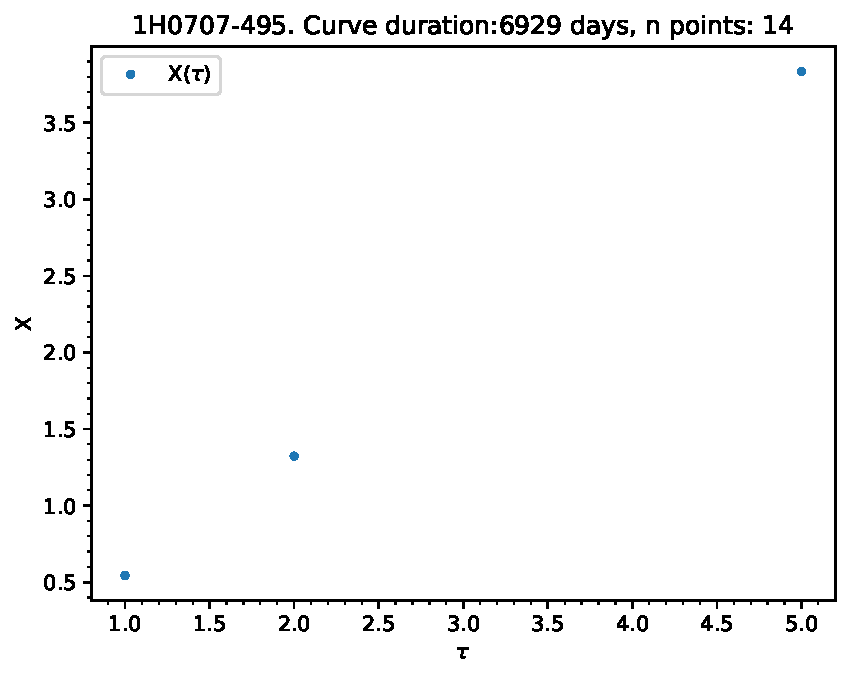
\includegraphics[width=0.49\textwidth]{Figs/Chapter5/X_tau_1H0707-495.pdf}  \hfill
  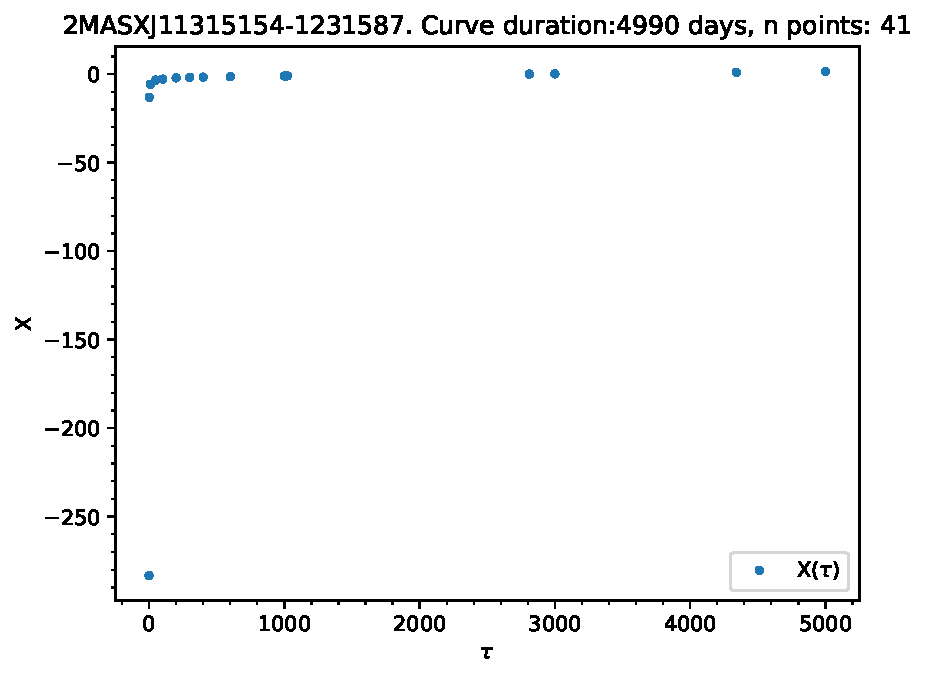
\includegraphics[width=0.49\textwidth]{Figs/Chapter5/X_tau_2MASXJ11315154-1231587.pdf} \\
  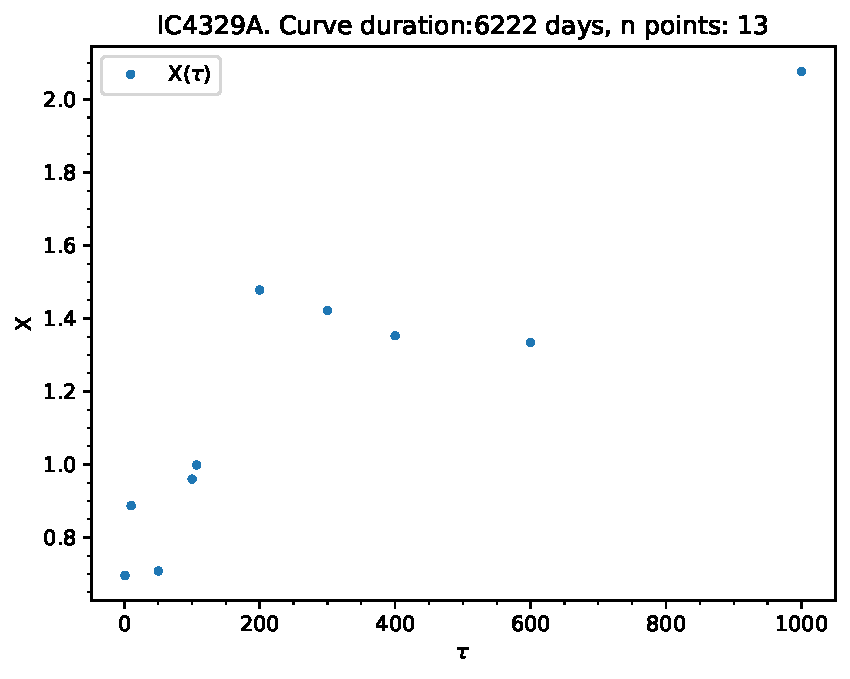
\includegraphics[width=0.49\textwidth]{Figs/Chapter5/X_tau_IC4329A.pdf} \hfill 
  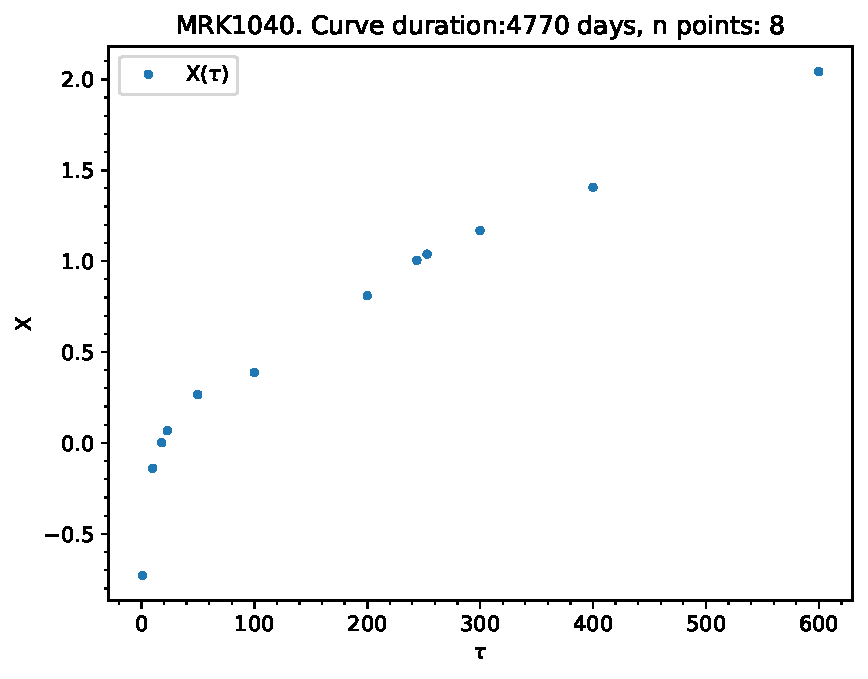
\includegraphics[width=0.49\textwidth]{Figs/Chapter5/X_tau_MRK1040.pdf}  \\ 
  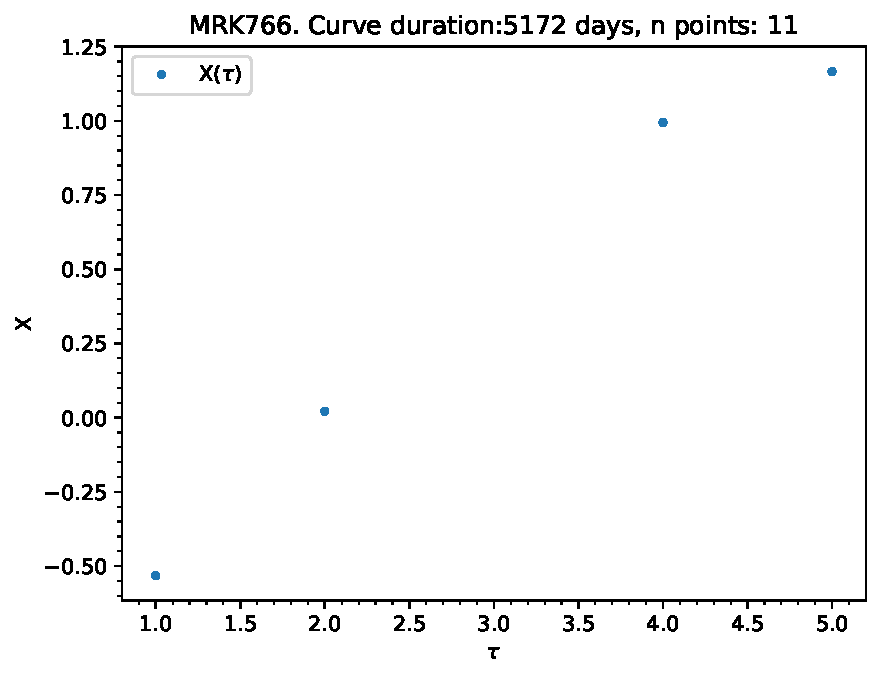
\includegraphics[width=0.49\textwidth]{Figs/Chapter5/X_tau_MRK766.pdf}  \hfill
  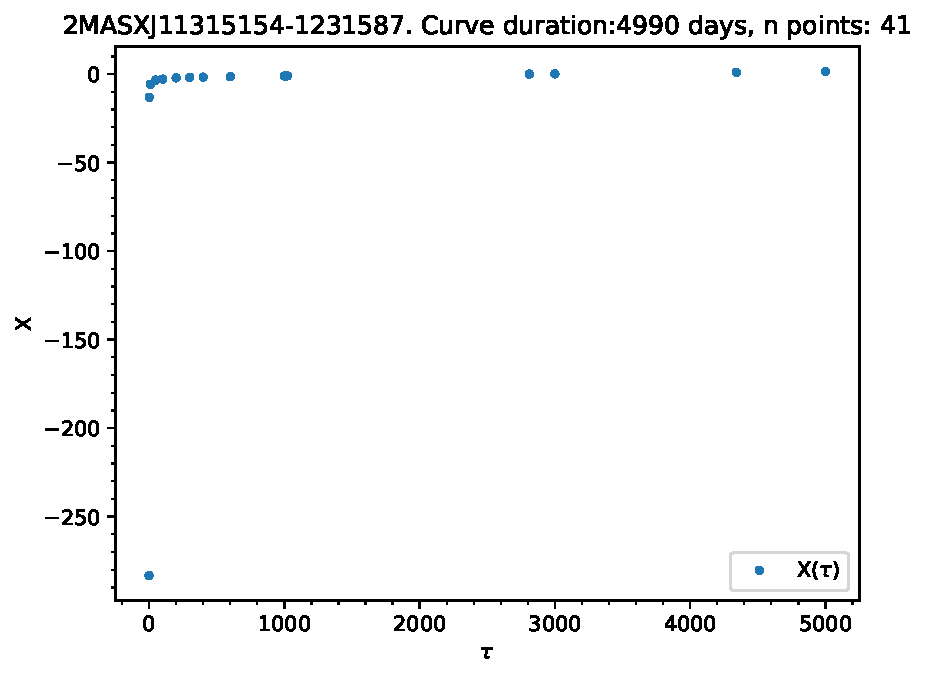
\includegraphics[width=0.49\textwidth]{Figs/Chapter5/X_tau_2MASXJ11315154-1231587.pdf} \\
  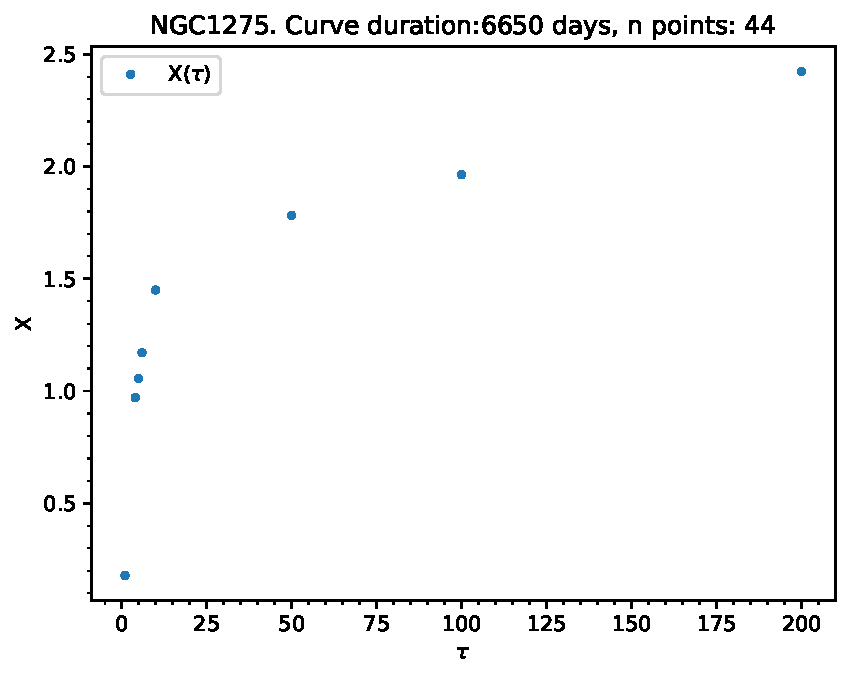
\includegraphics[width=0.49\textwidth]{Figs/Chapter5/X_tau_NGC1275.pdf} \hfill 
  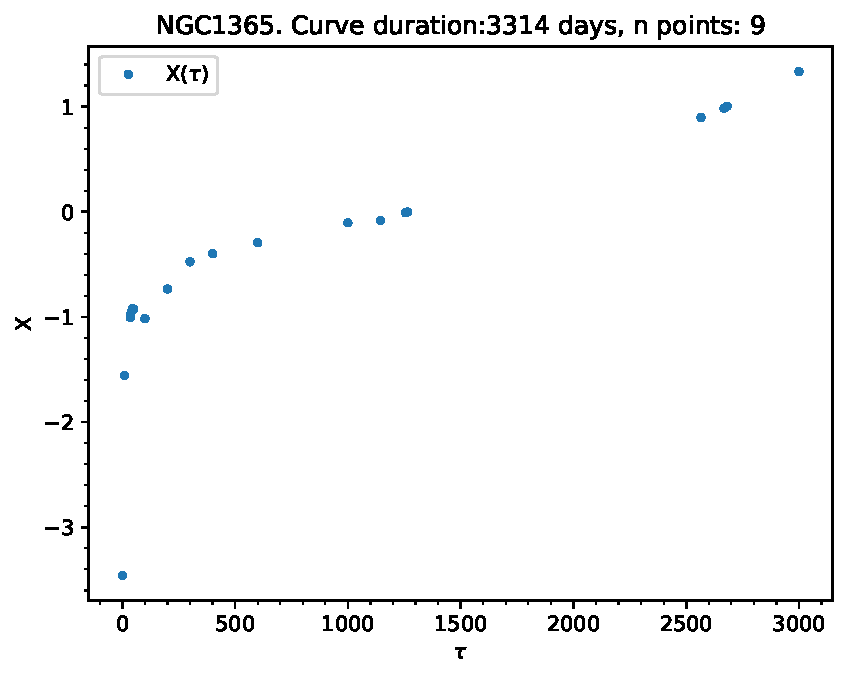
\includegraphics[width=0.49\textwidth]{Figs/Chapter5/X_tau_NGC1365.pdf} 
  \caption{X$(\tau)$ for our galaxy sample.}
    \label{fig:Xtau_1}
  }
\end{center}
\end{figure}

\begin{figure}
\begin{center}
    {
  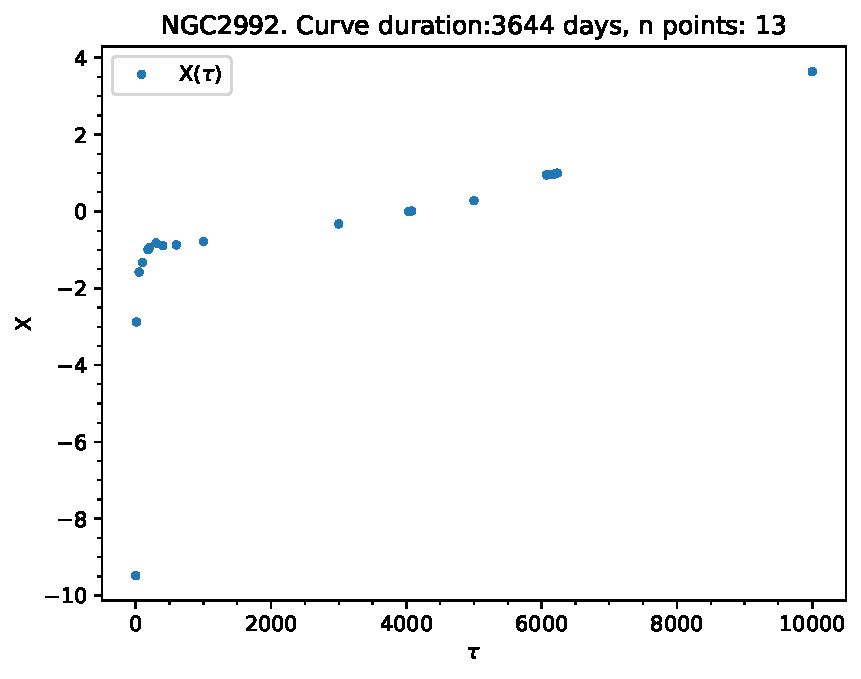
\includegraphics[width=0.49\textwidth]{Figs/Chapter5/X_tau_NGC2992.pdf}  \hfill
  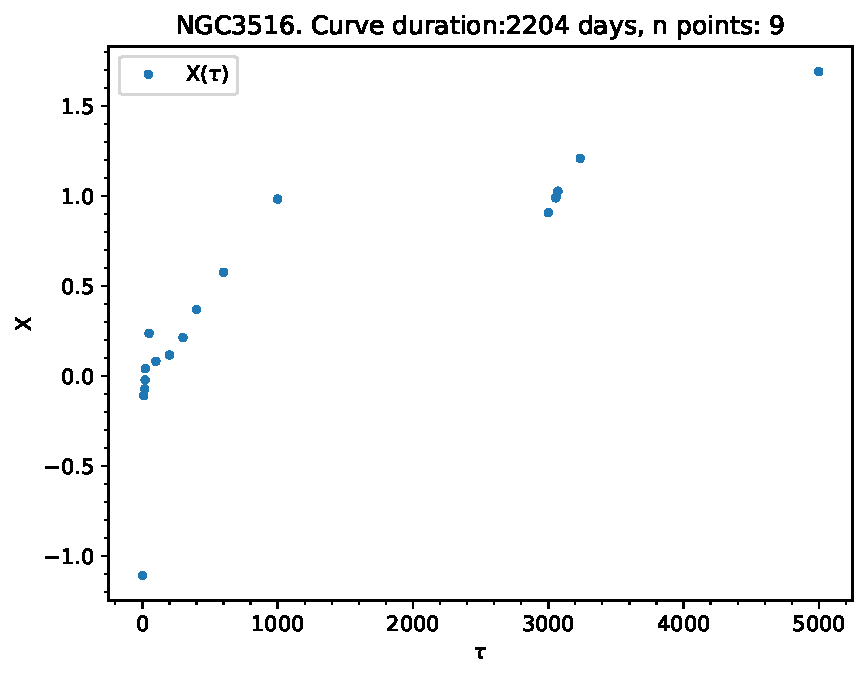
\includegraphics[width=0.49\textwidth]{Figs/Chapter5/X_tau_NGC3516.pdf} \\
  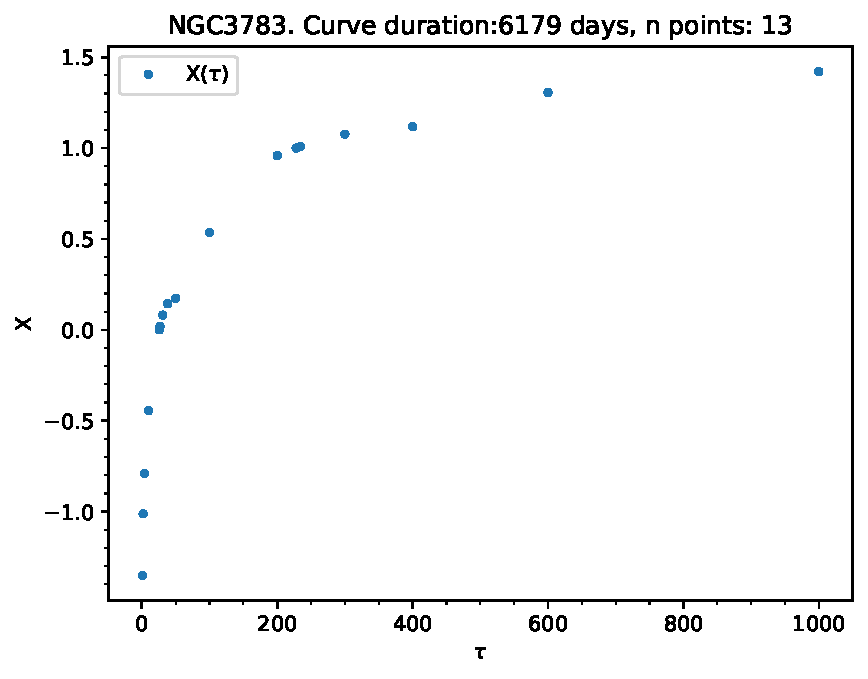
\includegraphics[width=0.49\textwidth]{Figs/Chapter5/X_tau_NGC3783.pdf} \hfill 
  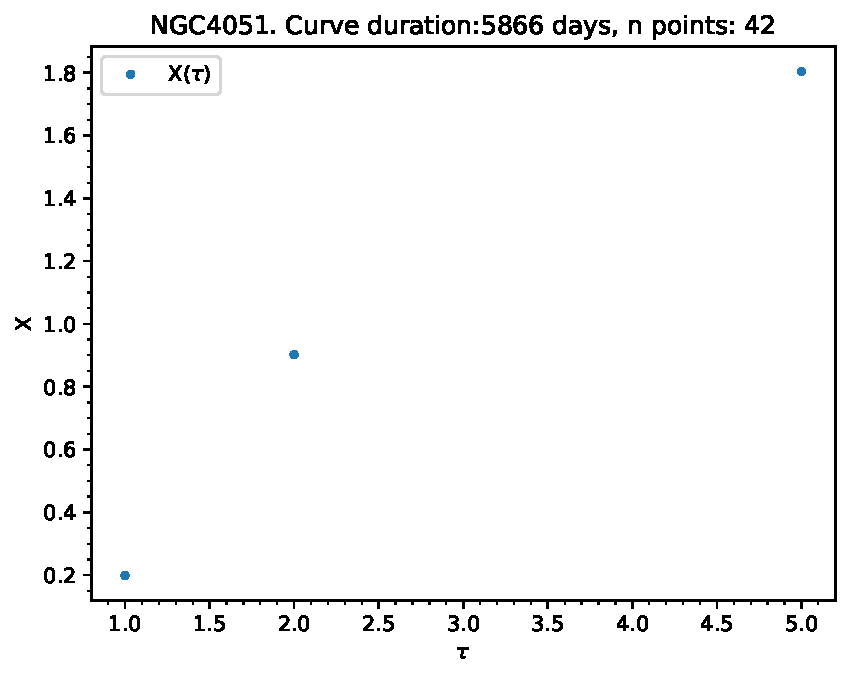
\includegraphics[width=0.49\textwidth]{Figs/Chapter5/X_tau_NGC4051.pdf}  \\ 
  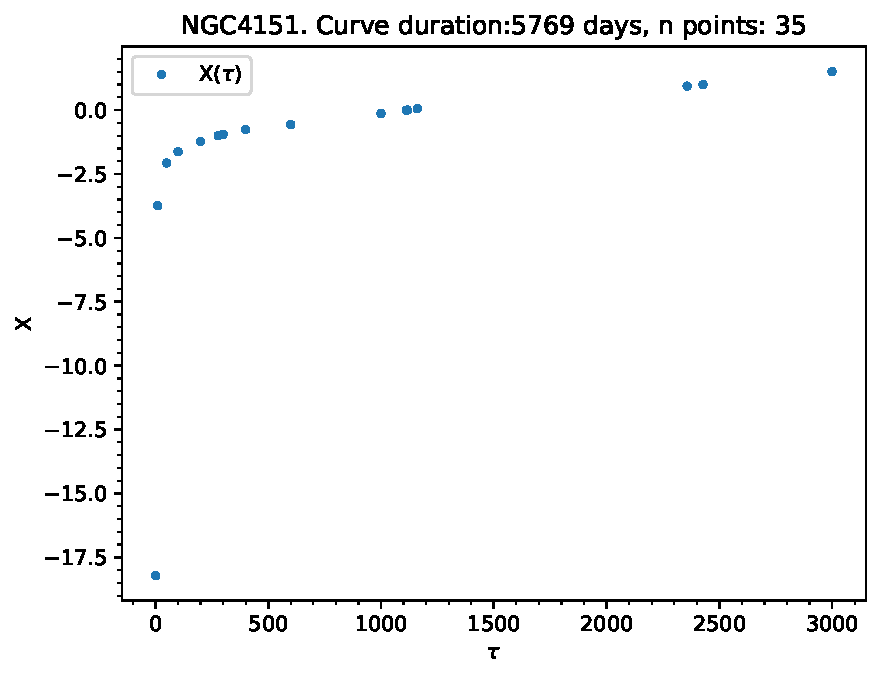
\includegraphics[width=0.49\textwidth]{Figs/Chapter5/X_tau_NGC4151.pdf}  \hfill
  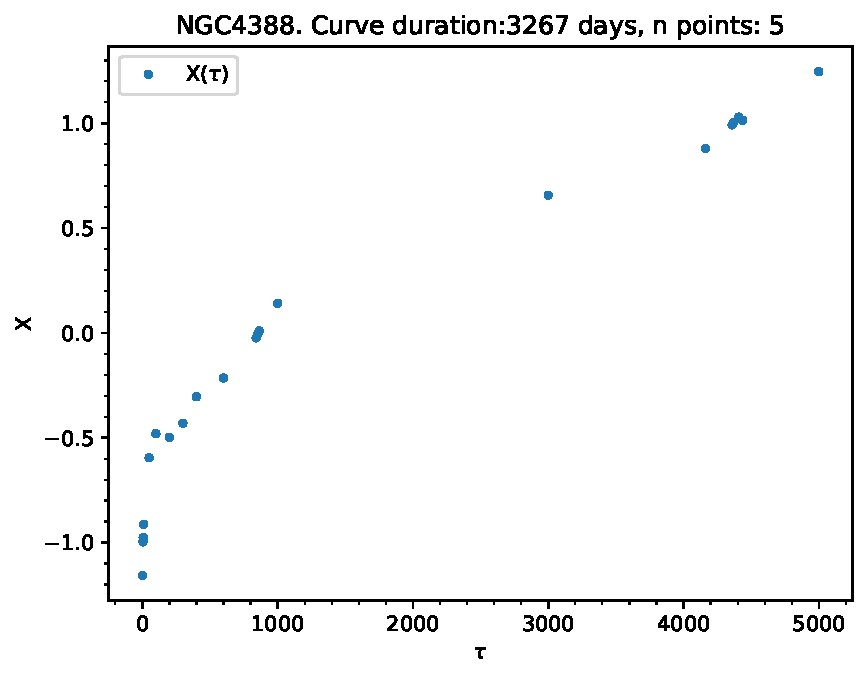
\includegraphics[width=0.49\textwidth]{Figs/Chapter5/X_tau_NGC4388.pdf} \\
  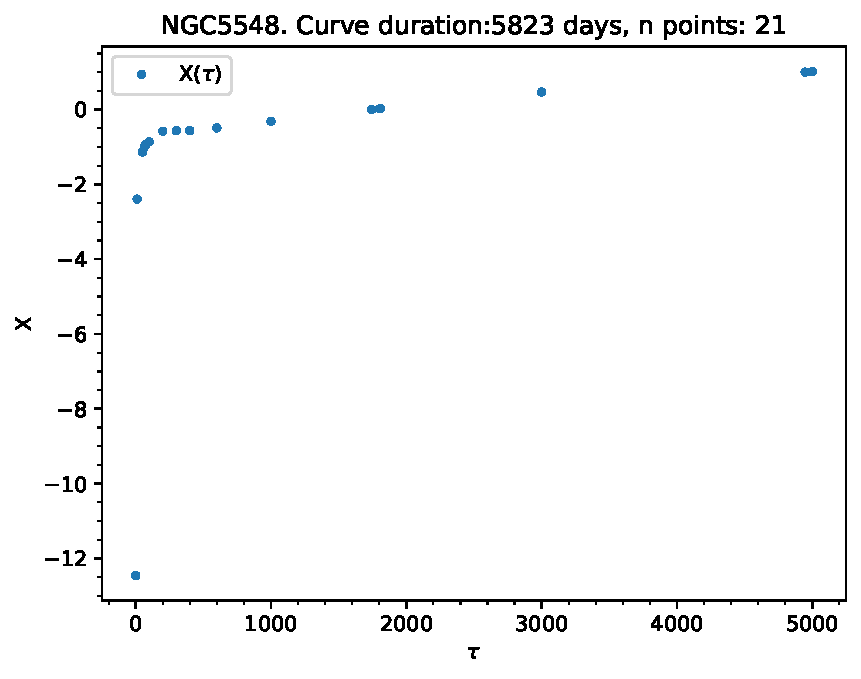
\includegraphics[width=0.49\textwidth]{Figs/Chapter5/X_tau_NGC5548.pdf} \hfill 
  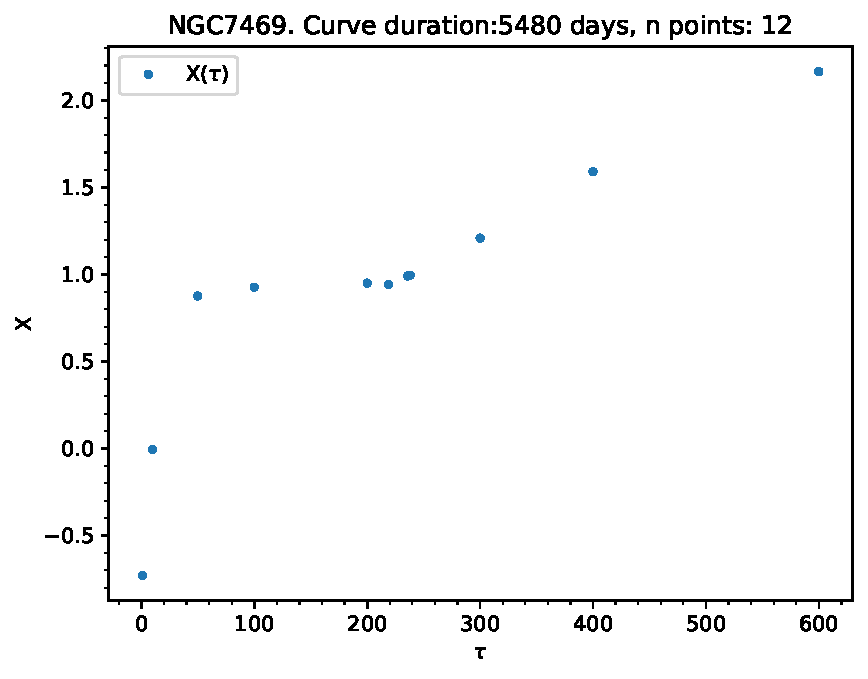
\includegraphics[width=0.49\textwidth]{Figs/Chapter5/X_tau_NGC7469.pdf}  
  \caption{Fig.~\ref{fig:Xtau_1} continued.}
    \label{fig:Xtau_2}
  }
\end{center}
\end{figure}

\begin{figure}
\begin{center}
    {
  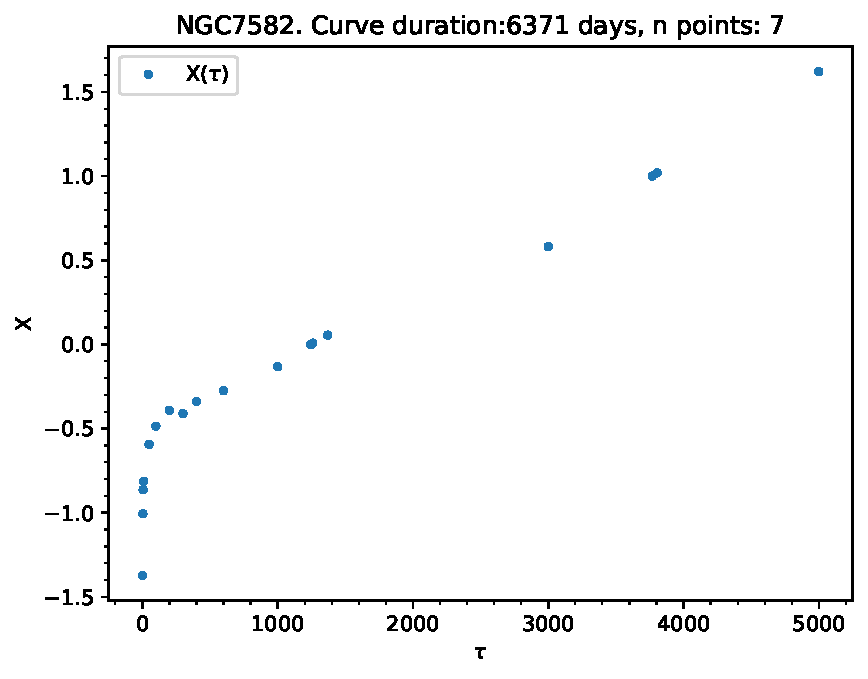
\includegraphics[width=0.49\textwidth]{Figs/Chapter5/X_tau_NGC7582.pdf}  \hfill
  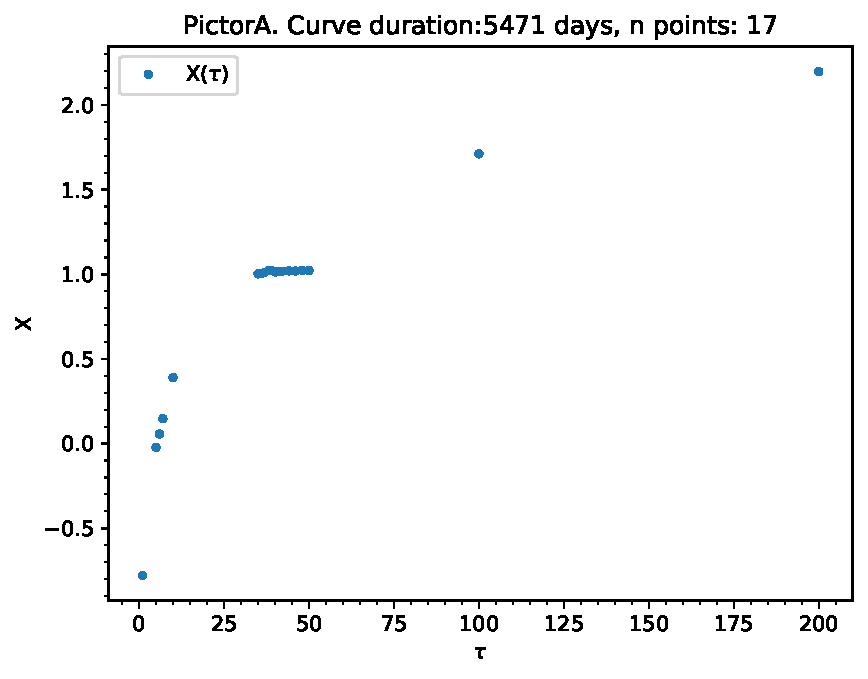
\includegraphics[width=0.49\textwidth]{Figs/Chapter5/X_tau_PictorA.pdf}
  \caption{Fig.~\ref{fig:Xtau_1} continued.}
    \label{fig:Xtau_3}
  }
\end{center}
\end{figure}

\section{Correlation between Fe line and continuum flux}
\section{Discussion}
\section{Conclusions}